% Created by tikzDevice version 0.12 on 2018-09-28 04:16:40
% !TEX encoding = UTF-8 Unicode
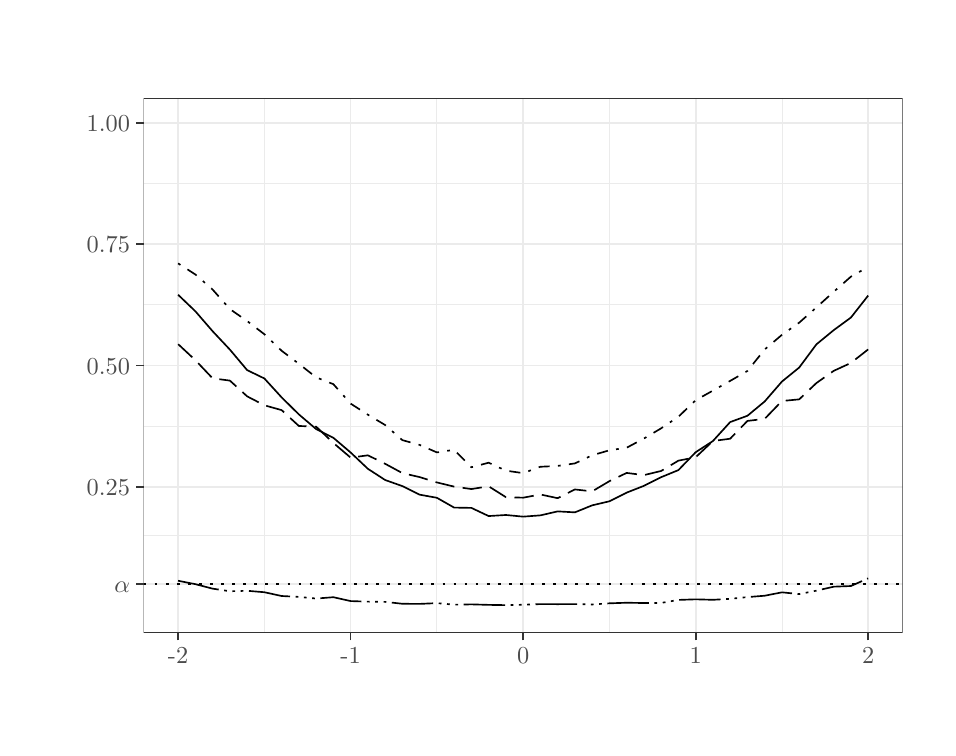
\begin{tikzpicture}[x=1pt,y=1pt]
\definecolor{fillColor}{RGB}{255,255,255}
\path[use as bounding box,fill=fillColor,fill opacity=0.00] (0,0) rectangle (325.21,252.94);
\begin{scope}
\path[clip] (  0.00,  0.00) rectangle (325.21,252.94);
\definecolor{drawColor}{RGB}{255,255,255}
\definecolor{fillColor}{RGB}{255,255,255}

\path[draw=drawColor,line width= 0.6pt,line join=round,line cap=round,fill=fillColor] (  0.00,  0.00) rectangle (325.21,252.94);
\end{scope}
\begin{scope}
\path[clip] ( 41.90, 34.26) rectangle (316.18,227.38);
\definecolor{fillColor}{RGB}{255,255,255}

\path[fill=fillColor] ( 41.90, 34.26) rectangle (316.18,227.38);
\definecolor{drawColor}{gray}{0.92}

\path[draw=drawColor,line width= 0.3pt,line join=round] ( 41.90, 69.37) --
	(316.18, 69.37);

\path[draw=drawColor,line width= 0.3pt,line join=round] ( 41.90,108.87) --
	(316.18,108.87);

\path[draw=drawColor,line width= 0.3pt,line join=round] ( 41.90,152.76) --
	(316.18,152.76);

\path[draw=drawColor,line width= 0.3pt,line join=round] ( 41.90,196.65) --
	(316.18,196.65);

\path[draw=drawColor,line width= 0.3pt,line join=round] ( 85.53, 34.26) --
	( 85.53,227.38);

\path[draw=drawColor,line width= 0.3pt,line join=round] (147.87, 34.26) --
	(147.87,227.38);

\path[draw=drawColor,line width= 0.3pt,line join=round] (210.21, 34.26) --
	(210.21,227.38);

\path[draw=drawColor,line width= 0.3pt,line join=round] (272.55, 34.26) --
	(272.55,227.38);

\path[draw=drawColor,line width= 0.6pt,line join=round] ( 41.90, 51.81) --
	(316.18, 51.81);

\path[draw=drawColor,line width= 0.6pt,line join=round] ( 41.90, 86.93) --
	(316.18, 86.93);

\path[draw=drawColor,line width= 0.6pt,line join=round] ( 41.90,130.82) --
	(316.18,130.82);

\path[draw=drawColor,line width= 0.6pt,line join=round] ( 41.90,174.71) --
	(316.18,174.71);

\path[draw=drawColor,line width= 0.6pt,line join=round] ( 41.90,218.60) --
	(316.18,218.60);

\path[draw=drawColor,line width= 0.6pt,line join=round] ( 54.37, 34.26) --
	( 54.37,227.38);

\path[draw=drawColor,line width= 0.6pt,line join=round] (116.70, 34.26) --
	(116.70,227.38);

\path[draw=drawColor,line width= 0.6pt,line join=round] (179.04, 34.26) --
	(179.04,227.38);

\path[draw=drawColor,line width= 0.6pt,line join=round] (241.38, 34.26) --
	(241.38,227.38);

\path[draw=drawColor,line width= 0.6pt,line join=round] (303.71, 34.26) --
	(303.71,227.38);
\definecolor{drawColor}{RGB}{0,0,0}

\path[draw=drawColor,line width= 0.6pt,dash pattern=on 1pt off 3pt on 4pt off 3pt ,line join=round] ( 54.37,167.76) --
	( 60.60,163.75) --
	( 66.83,158.31) --
	( 73.07,151.25) --
	( 79.30,146.93) --
	( 85.53,142.16) --
	( 91.77,136.19) --
	( 98.00,131.48) --
	(104.24,126.57) --
	(110.47,124.11) --
	(116.70,117.09) --
	(122.94,113.09) --
	(129.17,109.36) --
	(135.40,103.89) --
	(141.64,102.17) --
	(147.87, 99.46) --
	(154.10,100.41) --
	(160.34, 94.09) --
	(166.57, 95.74) --
	(172.81, 92.86) --
	(179.04, 91.98) --
	(185.27, 94.27) --
	(191.51, 94.58) --
	(197.74, 95.49) --
	(203.97, 98.41) --
	(210.21,100.23) --
	(216.44,101.15) --
	(222.68,104.48) --
	(228.91,108.17) --
	(235.14,112.35) --
	(241.38,118.32) --
	(247.61,121.79) --
	(253.84,125.30) --
	(260.08,128.89) --
	(266.31,136.65) --
	(272.55,141.95) --
	(278.78,146.34) --
	(285.01,151.85) --
	(291.25,157.50) --
	(297.48,162.98) --
	(303.71,166.49);

\path[draw=drawColor,line width= 0.6pt,dash pattern=on 15pt off 2pt on 1pt off 2pt on 1pt off 2pt on 1pt off 2pt ,line join=round] ( 54.37, 53.08) --
	( 60.60, 51.85) --
	( 66.83, 50.23) --
	( 73.07, 49.29) --
	( 79.30, 49.46) --
	( 85.53, 48.94) --
	( 91.77, 47.57) --
	( 98.00, 47.25) --
	(104.24, 46.65) --
	(110.47, 47.14) --
	(116.70, 45.74) --
	(122.94, 45.53) --
	(129.17, 45.46) --
	(135.40, 44.76) --
	(141.64, 44.72) --
	(147.87, 45.00) --
	(154.10, 44.44) --
	(160.34, 44.55) --
	(166.57, 44.37) --
	(172.81, 44.27) --
	(179.04, 44.41) --
	(185.27, 44.65) --
	(191.51, 44.62) --
	(197.74, 44.65) --
	(203.97, 44.51) --
	(210.21, 44.93) --
	(216.44, 45.14) --
	(222.68, 45.04) --
	(228.91, 45.07) --
	(235.14, 46.16) --
	(241.38, 46.37) --
	(247.61, 46.20) --
	(253.84, 46.55) --
	(260.08, 47.18) --
	(266.31, 47.67) --
	(272.55, 48.90) --
	(278.78, 48.27) --
	(285.01, 49.50) --
	(291.25, 50.94) --
	(297.48, 51.18) --
	(303.71, 53.96);

\path[draw=drawColor,line width= 0.6pt,dash pattern=on 7pt off 3pt ,line join=round] ( 54.37,138.58) --
	( 60.60,132.78) --
	( 66.83,126.22) --
	( 73.07,125.41) --
	( 79.30,119.72) --
	( 85.53,116.49) --
	( 91.77,114.74) --
	( 98.00,109.01) --
	(104.24,108.77) --
	(110.47,102.87) --
	(116.70, 97.57) --
	(122.94, 98.41) --
	(129.17, 95.35) --
	(135.40, 91.98) --
	(141.64, 90.54) --
	(147.87, 88.61) --
	(154.10, 87.10) --
	(160.34, 86.22) --
	(166.57, 87.21) --
	(172.81, 83.28) --
	(179.04, 83.10) --
	(185.27, 84.26) --
	(191.51, 82.92) --
	(197.74, 86.08) --
	(203.97, 85.38) --
	(210.21, 89.07) --
	(216.44, 92.05) --
	(222.68, 91.25) --
	(228.91, 92.76) --
	(235.14, 96.48) --
	(241.38, 97.71) --
	(247.61,103.57) --
	(253.84,104.41) --
	(260.08,110.84) --
	(266.31,111.58) --
	(272.55,118.04) --
	(278.78,118.63) --
	(285.01,124.53) --
	(291.25,128.92) --
	(297.48,131.80) --
	(303.71,136.68);

\path[draw=drawColor,line width= 0.6pt,line join=round] ( 54.37,156.41) --
	( 60.60,150.45) --
	( 66.83,143.25) --
	( 73.07,136.61) --
	( 79.30,129.20) --
	( 85.53,126.18) --
	( 91.77,119.34) --
	( 98.00,113.19) --
	(104.24,107.89) --
	(110.47,104.73) --
	(116.70, 99.43) --
	(122.94, 93.53) --
	(129.17, 89.49) --
	(135.40, 87.28) --
	(141.64, 84.19) --
	(147.87, 83.06) --
	(154.10, 79.52) --
	(160.34, 79.41) --
	(166.57, 76.46) --
	(172.81, 76.85) --
	(179.04, 76.25) --
	(185.27, 76.71) --
	(191.51, 78.15) --
	(197.74, 77.80) --
	(203.97, 80.33) --
	(210.21, 81.80) --
	(216.44, 84.93) --
	(222.68, 87.38) --
	(228.91, 90.51) --
	(235.14, 93.07) --
	(241.38, 99.53) --
	(247.61,103.57) --
	(253.84,110.42) --
	(260.08,112.70) --
	(266.31,117.86) --
	(272.55,125.06) --
	(278.78,130.12) --
	(285.01,138.51) --
	(291.25,143.63) --
	(297.48,148.20) --
	(303.71,156.13);

\path[draw=drawColor,line width= 0.6pt,dash pattern=on 1pt off 3pt ,line join=round] ( 41.90, 51.81) -- (316.18, 51.81);
\definecolor{drawColor}{gray}{0.20}

\path[draw=drawColor,line width= 0.6pt,line join=round,line cap=round] ( 41.90, 34.26) rectangle (316.18,227.38);
\end{scope}
\begin{scope}
\path[clip] (  0.00,  0.00) rectangle (325.21,252.94);
\definecolor{drawColor}{gray}{0.30}

\node[text=drawColor,anchor=base east,inner sep=0pt, outer sep=0pt, scale=  0.88] at ( 36.95, 48.78) {$\alpha$};

\node[text=drawColor,anchor=base east,inner sep=0pt, outer sep=0pt, scale=  0.88] at ( 36.95, 83.90) {$0.25$};

\node[text=drawColor,anchor=base east,inner sep=0pt, outer sep=0pt, scale=  0.88] at ( 36.95,127.79) {$0.50$};

\node[text=drawColor,anchor=base east,inner sep=0pt, outer sep=0pt, scale=  0.88] at ( 36.95,171.68) {$0.75$};

\node[text=drawColor,anchor=base east,inner sep=0pt, outer sep=0pt, scale=  0.88] at ( 36.95,215.57) {$1.00$};
\end{scope}
\begin{scope}
\path[clip] (  0.00,  0.00) rectangle (325.21,252.94);
\definecolor{drawColor}{gray}{0.20}

\path[draw=drawColor,line width= 0.6pt,line join=round] ( 39.15, 51.81) --
	( 41.90, 51.81);

\path[draw=drawColor,line width= 0.6pt,line join=round] ( 39.15, 86.93) --
	( 41.90, 86.93);

\path[draw=drawColor,line width= 0.6pt,line join=round] ( 39.15,130.82) --
	( 41.90,130.82);

\path[draw=drawColor,line width= 0.6pt,line join=round] ( 39.15,174.71) --
	( 41.90,174.71);

\path[draw=drawColor,line width= 0.6pt,line join=round] ( 39.15,218.60) --
	( 41.90,218.60);
\end{scope}
\begin{scope}
\path[clip] (  0.00,  0.00) rectangle (325.21,252.94);
\definecolor{drawColor}{gray}{0.20}

\path[draw=drawColor,line width= 0.6pt,line join=round] ( 54.37, 31.51) --
	( 54.37, 34.26);

\path[draw=drawColor,line width= 0.6pt,line join=round] (116.70, 31.51) --
	(116.70, 34.26);

\path[draw=drawColor,line width= 0.6pt,line join=round] (179.04, 31.51) --
	(179.04, 34.26);

\path[draw=drawColor,line width= 0.6pt,line join=round] (241.38, 31.51) --
	(241.38, 34.26);

\path[draw=drawColor,line width= 0.6pt,line join=round] (303.71, 31.51) --
	(303.71, 34.26);
\end{scope}
\begin{scope}
\path[clip] (  0.00,  0.00) rectangle (325.21,252.94);
\definecolor{drawColor}{gray}{0.30}

\node[text=drawColor,anchor=base,inner sep=0pt, outer sep=0pt, scale=  0.88] at ( 54.37, 23.25) {-2};

\node[text=drawColor,anchor=base,inner sep=0pt, outer sep=0pt, scale=  0.88] at (116.70, 23.25) {-1};

\node[text=drawColor,anchor=base,inner sep=0pt, outer sep=0pt, scale=  0.88] at (179.04, 23.25) {0};

\node[text=drawColor,anchor=base,inner sep=0pt, outer sep=0pt, scale=  0.88] at (241.38, 23.25) {1};

\node[text=drawColor,anchor=base,inner sep=0pt, outer sep=0pt, scale=  0.88] at (303.71, 23.25) {2};
\end{scope}
\end{tikzpicture}
